\section{Change of Variables} \label{S:11.9.Change_of_Variable}

\vspace*{-14 pt}
\framebox{\hspace*{3 pt}
\parbox{6.25 in}{\begin{goals}
\item What is a change of variables?
\item What is the Jacobian, and how is it related to a change of variables?
\end{goals}} \hspace*{3 pt}}

\subsection*{Introduction}

In single variable calculus, we encountered the idea of a change of variable in a definite integral through the method of substitution. For example, given the definite integral
\[\int_0^2 2x(x^2+1)^3 \, dx, \]
we naturally consider the change of variable $u = x^2+1$.  From this substitution, it follows that $du = 2x \, dx$, and since $x = 0$ implies $u = 1$ and $x = 2$ implies $u = 5$, we have transformed the original integral in $x$ into a new integral in $u$.  In particular,
\[\int_0^2 2x(x^2+1)^3 \, dx = \int_1^5 u^3 \, du.\]
The latter integral, of course, is far easier to evaluate.

Through our work with polar, cylindrical, and spherical coordinates, we have already implicitly seen some of the issues that arise in using a change of variables with two or three variables present.  In what follows, we seek to understand the general ideas behind any change of variables in a multiple integral.

\begin{pa} \label{PA:11.9} Consider the double integral
\begin{equation} \label{eq:11.9.COV_PA}
I = \iint_D x^2+y^2 \, dA,
\end{equation}
where $D$ is the upper half of the unit disk.
    \begin{enumerate}
    \item[(a)] Write the double integral $I$ given in Equation~(\ref{eq:11.9.COV_PA}) as an iterated integral in rectangular coordinates.

    \item[(b)] Write the double integral $I$ given in Equation~ (\ref{eq:11.9.COV_PA}) as an iterated integral in polar coordinates.


\end{enumerate}

\noindent When we write the double integral (\ref{eq:11.9.COV_PA}) as an iterated integral in polar coordinates we make a change of variables, namely
    \begin{equation}
x = r \cos(\theta)  \ \ \ \ \ \text{ and } \ \ \ \ \ y = r \sin(\theta).\label{eq:11.9.pol_to_rect}
\end{equation}
We also then have to change $dA$ to $r \, dr \, d\theta$. This process also identifies a ``polar rectangle'' $[r_1, r_2] \times [\theta_1, \theta_2]$ with the original Cartesian rectangle, under the transformation\footnote{A \emph{transformation} is another name for function:  here, the equations $x = r\cos(\theta)$ and $y = r\sin(\theta)$ define a function $T(r, \theta) = (r\cos(\theta), r\sin(\theta))$ so that $T$ is a function (transformation) from $\R^2$ to $\R^2$.  We view this transformation as mapping a version of the $x$-$y$ plane where the axes are viewed as representing $r$ and $\theta$ (the $r$-$\theta$ plane) to the familiar $x$-$y$ plane.} in Equation (\ref{eq:11.9.pol_to_rect}). The vertices of the polar rectangle are transformed into the vertices of a closed and bounded region in rectangular coordinates. 

\noindent To work with a numerical example, let's now consider the polar rectangle $P$ given by $[1, 2] \times [\frac{\pi}{6}, \frac{\pi}{4}]$, so that  $r_1 = 1$, $r_2=2$, $\theta_1 = \frac{\pi}{6}$, and $\theta_2 = \frac{\pi}{4}$. \\

    \begin{enumerate}
    \item[(c)] Use the transformation determined by the equations in~(\ref{eq:11.9.pol_to_rect}) to find the rectangular vertices that correspond to the polar vertices in the polar rectangle $P$. In other words, by substituting appropriate values of $r$ and $\theta$ into the two equations in~(\ref{eq:11.9.pol_to_rect}), find the values of the corresponding $x$ and $y$ coordinates for the vertices of the polar rectangle $P$. Label the point that corresponds to the polar vertex $(r_1, \theta_1)$ as $(x_1, y_1)$, the point corresponding to the polar vertex $(r_2, \theta_1)$ as $(x_2, y_2)$, the point corresponding to the polar vertex $(r_1, \theta_2)$ as $(x_3, y_3)$, and the point corresponding to the polar vertex $(r_2, \theta_2)$ as $(x_4, y_4)$.


    \item[(d)] Draw a picture of the figure in rectangular coordinates that has the points $(x_1,y_1)$, $(x_2,y_2)$, $(x_3, y_3)$, and $(x_4,y_4)$ as vertices. (Note carefully that because of the trigonometric functions in the transformation, this region will not look like a Cartesian rectangle.) What is the area of this region in rectangular coordinates? How does this area compare to the area of the original polar rectangle?

    \end{enumerate}
  

\end{pa}


\begin{activitySolution}
    \ba
    \item The double integral (\ref{eq:11.9.COV_PA}) can be evaluated in rectangular coordinates as the iterated integral
\[\int_{-1}^1 \int_{0}^{\sqrt{1-x^2}} x^2 + y^2 \, dy \, dx.\]


    \item By making the change of variables $x = r\cos(\theta)$ and $y = r\sin(\theta)$, and $dA = r \, dr \, d\theta$, we express the double integral (\ref{eq:11.9.COV_PA}) as the iterated integral
\[\int_0^{\pi} \int_0^1 r^2 r \, dr \, d\theta\]
in polar coordinates.

    \item Under the transformations in (\ref{eq:11.9.pol_to_rect})
\begin{itemize}
\item the vertex $(r_1, \theta_1) = \left(1, \frac{\pi}{6}\right)$ is sent to the point $(x_1, y_1) = \left(\frac{\sqrt{3}}{2}, \frac{1}{2}\right)$,
\item the vertex $(r_2, \theta_1) = \left(2, \frac{\pi}{6}\right)$ is sent to the point $(x_2, y_2) = \left(\sqrt{3}, 1 \right)$,
\item the vertex $(r_1, \theta_2) = \left(1, \frac{\pi}{4}\right)$ is sent to the point $(x_3, y_3) = \left(\frac{\sqrt{2}}{2}, \frac{\sqrt{2}}{2}\right)$,
\item the vertex $(r_2, \theta_2) = \left(2, \frac{\pi}{4}\right)$ is sent to the point $(x_4, y_4) = \left(\sqrt{2}, \sqrt{2}\right)$.
\end{itemize}

    \item If we lived in polar coordinates, the polar rectangle $P$ would look to us as shown below at left. The image $P'$ of the polar rectangle $P$ under the transformations in (\ref{eq:11.9.pol_to_rect}) is shown below at right.
%\begin{figure}[h]
\begin{center}
%\begin{minipage}{2.5in}
%\begin{center}
\resizebox{!}{2.4in}{\includegraphics{figures/fig_11_9_Polar_COV_1}}
%\end{center}
%\caption{Rectangle $P$ in the polar world.}
%\label{F:11.9.Change_vars1_a}
%\end{minipage}
\hspace{0.25in}
%\begin{minipage}{2.5in}
%\begin{center}
\resizebox{!}{2.4in}{\includegraphics{figures/fig_11_9_Polar_COV_2}}
%\end{center}
%\caption{Image $P'$ in the Cartesian world.}
%\label{F:11.9.Change_vars1_b}
%\end{minipage}
\end{center}
%\end{figure}
We have seen that the area of the transformed rectangle $P'$ is given by $\frac{r_2+r_1}{2} \Delta r \Delta \theta$, and as $\Delta r$ and $\Delta \theta$ go to 0 this area becomes the area element $dA = r \, dr \, d\theta$. This is the general idea of a change of variables in multiple integrals.

	\ea
	
\end{activitySolution}

 \afterpa 

\subsection*{Change of Variables in Polar Coordinates}

The general idea behind a change of variables is suggested by Preview Activity \ref{PA:11.9}.  There, we saw that in a change of variables from rectangular coordinates to polar coordinates, a polar rectangle $[r_1, r_2] \times [\theta_1, \theta_2]$ gets mapped to a Cartesian rectangle under the transformation
\begin{equation*}
x = r \cos(\theta)  \ \ \ \ \ \text{ and } \ \ \ \ \ y = r \sin(\theta).
\end{equation*}
The vertices of the polar rectangle $P$ are
transformed into the vertices 
of a closed and bounded region $P'$ in
rectangular coordinates. If we view the standard coordinate system as having the horizontal axis represent $r$ and the vertical axis represent $\theta$, then the polar
rectangle $P$ appears to us at left in Figure
\ref{F:11.9.Change_vars1_a}. The image $P'$ of the polar rectangle $P$
under the transformation given by (\ref{eq:11.9.pol_to_rect}) is shown at right in
Figure \ref{F:11.9.Change_vars1_a}.   We thus see that there is a correspondence between a simple region (a traditional, right-angled rectangle) and a more complicated region (a fraction of an annulus) under the function $T(r, \theta) = r\cos(\theta), r\sin(\theta))$.

\begin{figure}[ht]
\begin{center}
% \begin{minipage}{2.5in}
% \begin{center}
% \resizebox{!}{2.4in}{\includegraphics{11_9_Polar_COV_1}}
% \end{center}
% \caption{Rectangle $P$ in the polar world.}
% \end{minipage}
% \begin{minipage}{2.5in}
% \begin{center}
% \resizebox{!}{2.4in}{\includegraphics{11_9_Polar_COV_2}}
  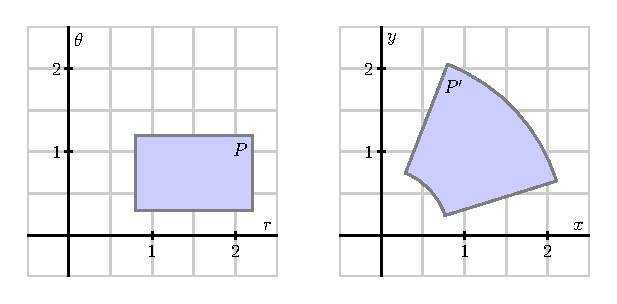
\includegraphics{figures/fig_11_9_polar_change.eps}
\end{center}
  \caption{A rectangle $P$ and its image $P'$.}
\label{F:11.9.Change_vars1_a}
% \end{minipage}
% \end{center}
\end{figure}
Furthermore, as Preview Activity~\ref{PA:11.9} suggest, it follows generally that for an original polar rectangle $P = [r_1, r_2] \times [\theta_1, \theta_2]$, the area of the transformed rectangle $P'$ is given by $\frac{r_2+r_1}{2} \Delta r \Delta \theta$.  Therefore, as $\Delta r$ and $\Delta \theta$ go to 0 this area becomes the familiar area element $dA = r \, dr \, d\theta$ in polar coordinates.  When we proceed to working with other transformations for different changes in coordinates, we have to understand how the transformation affects area so that we may use the correct area element in the new system of variables.

\subsection*{General Change of Coordinates}

We first focus on double integrals.  As with single integrals, we may be able to simplify a double integral of the form
\[\iint_D f(x,y) \, dA\]
by making a change of variables (that is, a substitution) of the form
\[x = x(s, t) \ \ \ \ \ \text{ and } \ \ \ \ \  y = y(s, t)\]
where $x$ and $y$ are functions of new variables $s$ and $t$. This transformation introduces a correspondence between a problem in the $xy$-plane and one in the the $st$-plane. The equations $x=x(s,t)$ and $y=y(s,t)$ convert $s$ and $t$ to $x$ and $y$; we call these formulas the \emph{change of variable} formulas. To complete the change to the new $s,t$ variables, we need to understand the area element, $dA$, in this new system.  The following activity helps to illustrate the idea.

\begin{activity} \label{A:11.9.1}  Consider the change of variables
\[x = s + 2 t \ \ \ \ \ \text{ and } \ \ \ \ \ y = 2 s + \sqrt{t}.\]
Let's see what happens to the rectangle $T = [0,1] \times [1,4]$ in the $st$-plane under this change of variable.
	\ba
	\item Draw a labeled picture of $T$ in the $st$-plane.
	
	\item Find the image of the $st$-vertex $(0,1)$ in the $xy$-plane.  Likewise, find the respective images of the other three vertices of the rectangle $T$: $(0,4)$, $(1,1)$, and $(1,4)$.	
	
	\item In the $xy$-plane, draw a labeled picture of the image, $T'$, of the original $st$-rectangle $T$. What appears to be the shape of the image, $T'$?
	
	\item To transform an integral with a change of variable,  we need to determine the area element $dA$ for image of the  transformed rectangle. How would find the area of the $xy$-figure $T'$? (Hint: Remember what the cross product of two vectors tells us.)
	
	\ea

\end{activity}
\begin{smallhint}

\end{smallhint}
\begin{bighint}

\end{bighint}
\begin{activitySolution}
\ba
\item A picture of the rectangle $T$ is shown in the image below.
\item The $st$-vertex $(0,1)$ gets sent to the point $(0+2(1), 2(0)+\sqrt{1}) = (2,1)$ in the $xy$-plane,
\item The point $(0,4)$ in the $st$-plane gets sent to the point $(8,2)$ in the $xy$-plane. The point $(1,1)$ in the $st$-plane gets sent to the point $(3,3)$ in the $xy$-plane.  The point $(1,4)$ in the $st$-plane gets sent to the point $(9,4)$ in the $xy$-plane.
\item The image $T'$ of $T$ is not a rectangle in the $xy$-plane because the change of variable formulas are not linear. The image $T'$ looks like a parallelogram. 
\item The area of $T'$ is the area of a parallelogram, which we can find with a cross product. The sides of the parallelogram can be viewed as the vectors $\vu = \langle 1, 2, 0\rangle$ and $\vv = \langle 6, 1, 0 \rangle$. The area of the parallelogram is then $|\vu \times \vv|$. 
\ea
\begin{center}
\resizebox{!}{1.0in}{\includegraphics{11_9_Act_1a}}
\end{center}

\end{activitySolution}
\aftera

Activity \ref{A:11.9.1} presents the general idea of how a change of variables works. We partition a rectangular domain in the $st$ system into subrectangles. Let $T = [a, b] \times [a+\Delta s, b+\Delta t]$ be one of these subrectangles. Then we transform this into a region $T'$ in the standard $xy$ Cartesian coordinate system. The region $T'$ is called the \emph{image} of $T$; the region $T$ is the \emph{pre-image} of $T'$.  Although the sides of this $xy$ region $T'$ aren't necessarily straight (linear), we will approximate the element of area $dA$ for this region with the area of the parallelogram whose sides are given by the vectors $\vv$ and $\vw$, where $\vv$ is the vector from $(x(a, b), y(a, b))$ to $(x(a + \Delta s, b), y(a + \Delta s, b))$, and $\vw$ is the vector from $(x(a, b), y(a, b))$ to $(x(a, b + \Delta t), y(a, b + \Delta t))$.

An example of an image $T'$ in the $xy$ plane that results from a transformation of a rectangle $T$ in the $st$ plane is shown in Figure \ref{F:11.9.Change_vars_ex}.
\begin{figure}[ht]
\begin{center}
%\resizebox{!}{2.5in}{\includegraphics{11_9_COV_area_element}}
  \includegraphics{figures/fig_11_9_general_change.eps}
\end{center}
\caption{Approximating an area of an image resulting from a transformation.}
\label{F:11.9.Change_vars_ex}
\end{figure}

The components of the vector $\vv$ are
\begin{align*}
\vv &= \left\langle x(a+ \Delta s, b) - x(a,b), y(a+ \Delta s, b) - y(a,b), 0 \right\rangle
\end{align*}
and similarly those for $\vw$ are
\begin{align*}
\vw &= \left\langle x(a, b+ \Delta t) - x(a,b), y(a, b+ \Delta s) - y(a,b), 0 \right\rangle.
\end{align*}

Slightly rewriting $\vv$ and $\vw$, we have 
\begin{align*}
\vv &= \left\langle \frac{x(a+ \Delta s, b) - x(a,b)}{\Delta s}, \frac{y(a+ \Delta s, b) - y(a,b)}{\Delta s}, 0 \right\rangle \Delta s, \ \mbox{and} \\
\vw &= \left\langle \frac{x(a, b+ \Delta t) - x(a,b)}{\Delta t}, \frac{y(a, b+ \Delta s) - y(a,b)}{\Delta t}, 0 \right\rangle \Delta t.
\end{align*}
For small $\Delta s$ and $\Delta t$, the definition of the partial derivative tells us that
\[\vv \approx \left\langle \frac{\partial x}{\partial s}(a,b), \frac{\partial y}{\partial s}(a,b), 0 \right\rangle \Delta s \ \ \ \ \ \text{ and } \ \ \ \ \  \vw \approx \left\langle \frac{\partial x}{\partial t}(a,b), \frac{\partial y}{\partial t}(a,b), 0 \right\rangle \Delta t.\]
Recall that the area of the parallelogram with sides $\vv$ and $\vw$ is the length of the cross product of the two vectors, $|\vv \times \vw|$. From this, we observe that
\begin{align*}
\vv \times \vw &\approx \left\langle \frac{\partial x}{\partial s}(a,b), \frac{\partial y}{\partial s}(a,b), 0 \right\rangle \Delta s \times \left\langle \frac{\partial x}{\partial t}(a,b), \frac{\partial y}{\partial t}(a,b), 0 \right\rangle \Delta t \\
    &= \left\langle 0, \ 0, \ \frac{\partial x}{\partial s}(a,b) \frac{\partial y}{\partial t}(a,b) - \frac{\partial x}{\partial t}(a,b) \frac{\partial y}{\partial s}(a,b) \right\rangle \Delta s \, \Delta t.
\end{align*}
Finally, by computing the magnitude of the cross product, we see that
\begin{align*}
|\vv \times \vw| &\approx \left|\left\langle 0,0, \frac{\partial x}{\partial s}(a,b) \frac{\partial y}{\partial t}(a,b) - \frac{\partial x}{\partial t}(a,b) \frac{\partial y}{\partial s}(a,b) \right\rangle \Delta s \, \Delta t\right| \\
    &= \left|\frac{\partial x}{\partial s}(a,b) \frac{\partial y}{\partial t}(a,b) - \frac{\partial x}{\partial t}(a,b) \frac{\partial y}{\partial s}(a,b)\right| \Delta s \, \Delta t.
\end{align*}

Therefore, as the number of subdivisions increases without bound in each direction, $\Delta s$ and $\Delta t$ both go to zero, and we have
\begin{equation} \label{E:Area_Element}
dA = \left|\frac{\partial x}{\partial s} \frac{\partial y}{\partial t} - \frac{\partial x}{\partial t} \frac{\partial y}{\partial s} \right| ds \, dt.
\end{equation}

Equation~\eqref{E:Area_Element} hence determines the general change of variable formula in a double integral, and we can now say that
\[\iint_T f(x,y) \, dA = \iint_R f(x,y) \, dy \, dx = \iint_{T'} f(x(s,t),y(s,t)) \left|\frac{\partial x}{\partial s} \frac{\partial y}{\partial t} - \frac{\partial x}{\partial t} \frac{\partial y}{\partial s}\right| ds \, dt.\]
The quantity
\[\left|\frac{\partial x}{\partial s} \frac{\partial y}{\partial t} - \frac{\partial x}{\partial t} \frac{\partial y}{\partial s}\right|\]
is called the \emph{Jacobian}\index{Jacobian}, and we denote the Jacobian using the shorthand notation 
\[ \left| \frac{\partial (x,y)}{\partial (s,t)} \right| =  \left| \frac{\partial x}{\partial s} \frac{\partial y}{\partial t} - \frac{\partial x}{\partial t} \frac{\partial y}{\partial s} \right|.\footnote{If you are familiar with determinants of matrices, we can can also represent $\frac{\partial (x,y)}{\partial (s,t)}$ as the determinant of a $2 \times 2$ matrix
\[\frac{\partial (x,y)}{\partial (s,t)} = \renewcommand{\tabcolsep}{0.1cm}
\renewcommand{\arraystretch}{2.5} \left| \begin{array}{cc} \ds \frac{\partial x}{\partial s} & \ds \frac{\partial x}{\partial t} \\ \ds \frac{\partial y}{\partial s} & \ds \frac{\partial y}{\partial t} \end{array} \right|.\]}\]

To summarize, the preceding change of variable formula that we have derived now follows.

\vspace*{5pt}
\nin \framebox{\hspace*{3 pt}
\parbox{6.25 in}{\textbf{Change of Variables in a Double Integral.\index{change of variable!double integral}} Suppose a change of variables $x = x(s,t)$ and $y = y(s,t)$ transforms a closed and bounded region $R$ in the $st$-plane into a closed and bounded region $R'$ in the $xy$-plane. Under modest conditions (that are studied in advanced calculus), it follows that
\[\iint_{R'} f(x,y) \, dA = \iint_{R} f(x(s,t), y(s,t)) \left|\frac{\partial (x,y)}{\partial (s,t)}\right| \, ds \, dt.\]
} \hspace*{3 pt}}
\vspace*{5pt}

\begin{activity} \label{A:11.9.2} Find the Jacobian when changing from rectangular to polar coordinates.  That is, for the transformation given by $x = r\cos(\theta)$, $y = r\sin(\theta)$, determine a simplified expression for the quantity 
$$\left|\frac{\partial x}{\partial r} \frac{\partial y}{\partial \theta} - \frac{\partial x}{\partial \theta} \frac{\partial y}{\partial r}\right|.$$
What do you observe about your result?  How is this connected to our earlier work with double integrals in polar coordinates?
\end{activity}
\begin{smallhint}

\end{smallhint}
\begin{bighint}

\end{bighint}
\begin{activitySolution}
In this case we have
\[x(r, \theta) = r \cos(\theta) \ \ \ \ \ \text{ and } \ \ \ \ \ y(r, \theta) = r \sin(\theta).\]
Since we can assume $r \geq 0$ in polar coordinates, the Jacobian is
\[\left|\frac{\partial x}{\partial r} \frac{\partial y}{\partial \theta} - \frac{\partial x}{\partial \theta} \frac{\partial y}{\partial r}\right| = \left|\cos(\theta)(r\cos(\theta)) - \sin(\theta)(r\sin(\theta))\right| = \left|r\cos^2(\theta) + r\sin^2(\theta)\right| = r\]
as expected.
\end{activitySolution}
\aftera


Given a particular double integral, it is natural to ask, ``how can we find a useful change of variables?'' There are two general factors to consider: if the integrand is particularly difficult, we might choose a change of variables that would make the integrand easier; or, given a complicated region of integration, we might choose a change of variables that transforms the region of integration into one that has a simpler form. These ideas are illustrated in the next activities.

\begin{activity} \label{A:11.9.3} Consider the problem of finding the area of the region $D'$ defined by the ellipse $x^2 + \frac{y^2}{4} = 1$. Here we will make a change of variables so that the pre-image of the domain is a circle.
	\ba
	\item Let $x(s,t) = s$ and $y(s,t) = 2t$. Explain why the pre-image of the original ellipse (which lies in the $xy$ plane)   is the circle $s^2 + t^2 = 1$ in the $st$-plane.
	
	\item Recall that the area of the ellipse $D'$ is determined by the double integral $\ds \iint_{D'} 1 \, dA$. Explain why
	\[\iint_{D'} 1 \, dA = \iint_{D} 2 \, ds \, dt\]
	where $D$ is the disk bounded by the circle $s^2 + t^2 = 1$.  In particular, explain the source of the ``2'' in the $st$ integral.
	
	\item Without evaluating any of the integrals present, explain why the area of the original elliptical region $D'$ is $2\pi$.

	

	\ea

\end{activity}
\begin{smallhint}

\end{smallhint}
\begin{bighint}

\end{bighint}
\begin{activitySolution}
	\ba
	\item Substituting $s$ for $x$ and $2t$ for $y$ in our ellipse equation gives us
\[1 = x^2 + \frac{y^2}{4} = s^2 + \frac{(2t)^2}{4} = s^2 + t^2.\]
So the pre-image of the the ellipse in the $st$-plane is the circle $s^2 + t^2 = 1$.
	
	\item This is just asking us to find the Jacobian
\[\left|\frac{\partial(x,y)}{\partial(s,t)}\right| = \left|\frac{\partial x}{\partial s} \frac{\partial y}{\partial t} - \frac{\partial x}{\partial t} \frac{\partial y}{\partial s}\right| = |(1)(2) - (0)(0)| = 2.\]
	
	\item We know that $D'$ is a circle of radius 1 and so has area $\pi$. Therefore, 
\[\iint_D 1 \, dA = \iint_{D'} 2 \, ds \, dt = 2\iint_{D'}  \, ds \, dt = 2\pi.\]

	\ea
\end{activitySolution}
\aftera


\begin{activity} \label{A:11.9.4} Let $D'$ be the region in the $xy$-plane bounded by the lines $y=0$, $x=0$, and $x+y=1$. We will evaluate the double integral
\begin{equation}
\iint_{D'} \sqrt{x+y}(x-y)^2 \, dA \label{eq:11.9.COV_ex}
\end{equation}
with a change of variables.
	\ba
	\item Sketch the region $D'$ in the $xy$ plane.
	
	\item We would like to make a substitution that makes the integrand easier to antidifferentiate. Let $s = x+y$ and $t = x-y$. Explain why this should make antidifferentiation easier by making the corresponding substitutions and writing the new integrand in terms of $s$ and $t$.

	\item Solve the equations $s = x+y$ and $t = x-y$ for $x$ and $y$. (Doing so determines the standard form of the transformation, since we will have $x$ as a function of $s$ and $t$, and $y$ as a function of $s$ and $t$.)

	\item To actually execute this change of variables, we need to know the $st$-region $D$ that corresponds to the $xy$-region $D'$.
		\begin{enumerate}[i.]
		\item What $st$ equation corresponds to the $xy$ equation $x+y=1$?
		
		\item What $st$ equation corresponds to the $xy$ equation $x=0$?
		
		\item What $st$ equation corresponds to the $xy$ equation $y=0$?
		
		\item Sketch the $st$ region $D$ that corresponds to the $xy$ domain $D'$.
			
		\end{enumerate}
		
	\item Make the change of variables indicated by $s = x+y$ and $t = x-y$ in the double integral (\ref{eq:11.9.COV_ex}) and set up an iterated integral in $st$ variables whose value is the original given double integral. Finally, evaluate the iterated integral.
	
	
	
	\ea

\end{activity}
\begin{smallhint}

\end{smallhint}
\begin{bighint}

\end{bighint}
\begin{activitySolution}
	\ba
	\item A sketch of the $xy$ domain $D'$ is shown below.
			
	\item This change of variable would make the integrand look like $\sqrt{s}t^2$, which separates the variables and makes the integration easier. 
	

	\item A little algebra shows that $x = \frac{1}{2}(s+t)$ and $y = \frac{1}{2}(s-t)$.


	\item To make this change of variables, we will need to know the $st$-region $S$ that corresponds to the $xy$-region $D$.
		\begin{enumerate}[i.]
		\item Using our change of variables we have 
\[1 = x+y = \frac{1}{2}((s+t)+(s-t)) = s.\]
	
		\item Using our change of variables we have 
\[0 = x = \frac{1}{2}(s+t)\]
or
\[s+t = 0.\]		
		\item Using our change of variables we have 
\[0 = y = \frac{1}{2}(s-t)\]
or
\[s-t = 0.\]
	
		\item The region $D$ is shown below. 
		
		\end{enumerate}
		
	\item We need the Jacobian
\[\left|\frac{\partial(x,y)}{\partial(s,t)}\right| = \left|\frac{\partial x}{\partial s} \frac{\partial y}{\partial t} - \frac{\partial x}{\partial t} \frac{\partial y}{\partial s}\right| = \left| \left(\frac{1}{2}\right)\left(-\frac{1}{2}\right) - \left(\frac{1}{2}\right)\left(\frac{1}{2}\right)\right| = \frac{1}{2}.\]
Then
\begin{align*}
\iint_D \sqrt{x+y}(x-y)^2 \, dA &= \iint_S \sqrt{s}t^2 \left|\frac{\partial(x,y)}{\partial(s,t)}\right| \, ds \, dt \\
	&= \int_0^1 \int_{-s}^{s} \sqrt{s}t^2 \frac{1}{2} \, dt \, ds \\
	&= \frac{1}{2} \int_0^1 \left. \sqrt{s} \frac{t^3}{3} \right|_{-s}^{s} \, ds \\
	&= \frac{1}{3} \int_0^1 \sqrt{s}s^3 \, ds \\
	&= \frac{1}{3} \int_0^1 s^{7/2} \, ds \\
	&= \frac{2}{27} \left. s^{9/2} \right|_0^1 \\
	&= \frac{2}{27}.
\end{align*}
	\ea
\begin{center}
\resizebox{!}{1.5in}{\includegraphics{11_9_Act_4}}
\end{center}
\end{activitySolution}
\aftera



\subsection*{Change of Variables in a Triple Integral}

Given a function $f = f(x,y,z)$ over a region $S'$ in $\R^3$, similar arguments can be used to show that a change of variables $x=x(s,t,u)$, $y=y(s,t,u)$, and $z = z(s,t,u)$ in a triple integral\index{change of variable!triple integral} results in the equality
\[\iiint_{S'} f(x,y,z) \, dV = \iiint_{S} f(x(s,t,u),y(s,t,u),z(s,t,u)) \ \left| \frac{\partial(x,y,z)}{\partial(s,t,u)} \right| \, ds \, dt \, du,\]
where
\[\frac{\partial(x,y,z)}{\partial(s,t,u)} = \left| \renewcommand{\tabcolsep}{0.1cm}
\renewcommand{\arraystretch}{2.5}
\begin{array}{ccc} \ds \frac{\partial x}{\partial s} & \ds \frac{\partial x}{\partial t} & \ds \frac{\partial x}{\partial u} \\ \ds \frac{\partial y}{\partial s} & \ds \frac{\partial y}{\partial t} & \ds \frac{\partial y}{\partial u} \\ \ds \frac{\partial z}{\partial s} & \ds \frac{\partial z}{\partial t} & \ds \frac{\partial z}{\partial u} \end{array} \right|.\]
In expanded form,
\[\frac{\partial(x,y,z)}{\partial(s,t,u)} = \frac{\partial x}{\partial s}\left[\frac{\partial y}{\partial t}\frac{\partial z}{\partial u} - \frac{\partial y}{\partial u}\frac{\partial z}{\partial t}\right] - \frac{\partial x}{\partial t}\left[\frac{\partial y}{\partial s}\frac{\partial z}{\partial u} - \frac{\partial y}{\partial u}\frac{\partial z}{\partial s}\right] + \frac{\partial x}{\partial u}\left[\frac{\partial y}{\partial s}\frac{\partial z}{\partial t} - \frac{\partial y}{\partial t}\frac{\partial z}{\partial s}\right].\]
The expression $\left|\frac{\partial(x,y,z)}{\partial(s,t,u)}\right|$ is again called the Jacobian\index{Jacobian}.

%\begin{activity} \label{A:11.9.5} Verify that the change of variables
\[x(\rho, \theta, \phi) = \rho \sin(\phi) \cos(\theta), \ \ \ \ \ y(\rho, \theta, \phi) = \rho \sin(\phi) \sin(\theta), \ \ \ \ \ z(\rho, \theta, \phi) = \rho \cos(\phi)\]
from spherical coordinates to rectangular coordinates has Jacobian $\rho^2 \sin(\phi)$.

\end{activity}
\begin{smallhint}

\end{smallhint}
\begin{bighint}

\end{bighint}
\begin{activitySolution}
\begin{align*}
\left|\frac{\partial(x,y,z)}{\partial(\rho,\theta,\phi)}\right| &= \left|\frac{\partial x}{\partial \rho}\left[\frac{\partial y}{\partial \theta}\frac{\partial z}{\partial \phi} - \frac{\partial y}{\partial \phi}\frac{\partial z}{\partial \theta}\right] - \frac{\partial x}{\partial \theta}\left[\frac{\partial y}{\partial \rho}\frac{\partial z}{\partial \phi} - \frac{\partial y}{\partial \phi}\frac{\partial z}{\partial \rho}\right] + \frac{\partial x}{\partial \phi}\left[\frac{\partial y}{\partial \rho}\frac{\partial z}{\partial \theta} - \frac{\partial y}{\partial \theta}\frac{\partial z}{\partial \rho}\right]\right| \\
	&= \left|\sin(\phi)\cos(\theta)[(\rho\sin(\phi)\cos(\theta))(-\rho \sin(\phi)) - (\rho \cos(\phi) \sin(\theta))(0)] \right. \\
	& \qquad + \rho \sin(\phi) \sin(\theta)[(\sin(\phi)\sin(\theta))(-\rho \sin(\phi)) - (\rho \cos(\phi) \sin(\theta))(\cos(\phi))] \\
	& \qquad + \left. \rho \cos(\phi) \cos(\theta)[(\sin(\phi)\sin(\theta))(0) - (\rho \sin(\phi) \cos(\theta))(\cos(\phi))]\right| \\
	&= \left|-\rho^2 \sin^3(\phi) \cos^2(\theta) - \rho^2 \sin^3(\phi) \sin^2(\theta) \right.\\
	& \qquad - \left. \rho^2 \sin(\phi)\cos^2(\phi) \sin^2(\theta) - \rho^2 \sin(\phi) \cos^2(\phi) \cos^2(\theta) \right| \\
	&= \left| -\rho^2 [ \sin^3(\phi) + \sin(\phi) \cos^2(\phi)] \right| \\
	&= \left|-\rho^2 [ \sin^3(\phi) + \sin(\phi) (1-\sin^2(\phi))] \right| \\
	&= \rho^2 \sin(\phi).
\end{align*}
\end{activitySolution}
\aftera


\begin{summary}
\item If an integral is described in terms of one set of variables, we may write that set of variables in terms of another set of the same number of variables. If the new variables are chosen appropriately, the transformed integral may be easier to evaluate. 
\item The Jacobian is a scalar function that relates the area or volume element in one coordinate system to the corresponding element in a new system determined by a change of variables. 
\end{summary}

\nin \hrulefill

\begin{exercises} 

\item Let $D'$ be the region in the $xy$ plane that is the parallelogram with vertices $(3,3)$, $(4,5)$, $(5,4)$, and $(6,6)$.
	\ba
	 	\item Sketch and label the region $D'$ in the $xy$ plane. 
		\item Consider the integral $\iint_{D'} (x+y) \, dA$.  Explain why this integral would be difficult to set up as an iterated integral.
		\item Let a change of variables be given by $x = 2u + v$, $y = u + 2v$.  Using substitution or elimination, solve this system of equations for $u$ and $v$ in terms of $x$ and $y$.
		\item Use your work in (c) to find the pre-image, $D$, which lies in the $uv$ plane, of the originally given region $D'$, which lies in the $xy$ plane.  For instance, what $uv$ point corresponds to $(3,3)$ in the $xy$ plane?
		\item Use the change of variables in (c) and your other work to write a new iterated integral in $u$ and $v$ that is equivalent to the original $xy$ integral $\iint_{D'} (x+y) \, dA$.
		\item Finally, evaluate the $uv$ integral, and write a sentence to explain why the change of variables made the integration easier.
	\ea

%	\item Find the $z$-coordinate of the center of mass of the solid that lies between the hemisphere of radius 2 and the hemisphere of radius 1, each of which are bounded below by the plane $z=0$.  Assume that the density of the solid is given by the function $d(x,y,z)=x^2+y^2+z^2$.  Can you find $\overline{x}$ and $\overline{y}$ without integrating?

\begin{exerciseSolution}
	\ba
	 	\item The region $D'$ is a parallelogram. 
		\item Since the boundaries of $D'$ change in both the $x$ and $y$ directions, integrating with respect to either $x$ or $y$ would require multiple integrals. 
		\item Multiplying both sides of $y=u+2v$ and subtracting corresponding sides of $x = 2u + v$ leaves us with $2y-x = 3v$. So $v = \frac{1}{3}(2y-x)$. Multiplying both sides of $x = 2u + v$ and subtracting corresponding sides of $y=u+2v$ leaves us with $2x-y = 3v$. So $u = \frac{1}{3}(2x-y)$.
		\item The vertex $(3,3)$ of the region $D'$ corresponds to the point $\left(\frac{1}{3}(2(3)-3), \frac{1}{3}(2(3)-3)\right) = (1,1)$ in $D$. Similarly, the points $(4,5)$, $(5,4)$, and $(6,6)$ in $D'$ correspond to the points $(1,2)$, $(2,1)$, and $(2,2)$, respectively, in $D$. So the pre-image $D$ is the square with vertices $(1,1)$, $(1,2)$, $(2,1)$, and $(2,2)$. 
		\item For our change of variables we have 
\[\left|\frac{\partial (x,y)}{\partial (u,v)}\right| = \left| \frac{\partial x}{\partial u} \frac{\partial y}{\partial v} - \frac{\partial y}{\partial u} \frac{\partial x}{\partial v} \right| = \left|(2)(2) - (1)(1) \right| = 3.\]
Using the change of variables in (c) we have that  
\[\iint_{D'} (x+y) \, dA = \iint_{D} (3u+3v) \left|\frac{\partial (x,y)}{\partial (u,v)}\right| \, dA = \int_{1}^{2} \int_{1}^{2} 3(3u+3v) \, dv \, du.\]
		\item The $uv$ integral evaluates to 
\begin{align*}
\int_{1}^{2} \int_{1}^{2} 3(3u+3v) \, dv \, du &= 9\int_{1}^{2}  \left(uv+\frac{1}{2}v^2\right)\biggm|_{1}^{2}  \, du \\
	&= 9\int_{1}^{2}  \left(u+\frac{3}{2}\right)  \, du \\
	&= 9\left(\frac{1}{2}u^2+\frac{3}{2}u\right)\biggm|_{1}^{2} \\
	&= 9\left(\frac{1}{2}u^2+\frac{3}{2}u\right)\biggm|_{1}^{2} \\
	&= 27.
\end{align*}
	\ea
\end{exerciseSolution}

\item Consider the change of variables
\[x(\rho, \theta, \phi) = \rho \sin(\phi) \cos(\theta) \ \ \ \ \ y(\rho, \theta, \phi) = \rho \sin(\phi) \sin(\theta) \ \ \ \ \ z(\rho, \theta, \phi) = \rho \cos(\phi),\]
which is the transformation from spherical coordinates to rectangular coordinates.  Determine the Jacobian of the transformation.  How is the result connected to our earlier work with iterated integrals in spherical coordinates?

\begin{exerciseSolution}
Here we have 
\begin{align*}
\left|\frac{\partial(x,y,z)}{\partial(\rho,\theta,\phi)}\right| &= \left|\frac{\partial x}{\partial \rho}\left[\frac{\partial y}{\partial \theta}\frac{\partial z}{\partial \phi} - \frac{\partial y}{\partial \phi}\frac{\partial z}{\partial \theta}\right] - \frac{\partial x}{\partial \theta}\left[\frac{\partial y}{\partial \rho}\frac{\partial z}{\partial \phi} - \frac{\partial y}{\partial \phi}\frac{\partial z}{\partial \rho}\right] + \frac{\partial x}{\partial \phi}\left[\frac{\partial y}{\partial \rho}\frac{\partial z}{\partial \theta} - \frac{\partial y}{\partial \theta}\frac{\partial z}{\partial \rho}\right]\right| \\
	&= \left|\sin(\phi)\cos(\theta)[(\rho\sin(\phi)\cos(\theta))(-\rho \sin(\phi)) - (\rho \cos(\phi) \sin(\theta))(0)] \right. \\
	& \qquad + \rho \sin(\phi) \sin(\theta)[(\sin(\phi)\sin(\theta))(-\rho \sin(\phi)) - (\rho \cos(\phi) \sin(\theta))(\cos(\phi))] \\
	& \qquad + \left. \rho \cos(\phi) \cos(\theta)[(\sin(\phi)\sin(\theta))(0) - (\rho \sin(\phi) \cos(\theta))(\cos(\phi))]\right| \\
	&= \left|-\rho^2 \sin^3(\phi) \cos^2(\theta) - \rho^2 \sin^3(\phi) \sin^2(\theta) \right.\\
	& \qquad - \left. \rho^2 \sin(\phi)\cos^2(\phi) \sin^2(\theta) - \rho^2 \sin(\phi) \cos^2(\phi) \cos^2(\theta) \right| \\
	&= \left| -\rho^2 [ \sin^3(\phi) + \sin(\phi) \cos^2(\phi)] \right| \\
	&= \left|-\rho^2 [ \sin^3(\phi) + \sin(\phi) (1-\sin^2(\phi))] \right| \\
	&= \rho^2 \sin(\phi).
\end{align*}
This is exactly the volume element in spherical coordinates that we derived earlier. 
\end{exerciseSolution}

	\item In this problem, our goal is to find the volume of the ellipsoid $\frac{x^2}{a^2} + \frac{y^2}{b^2} + \frac{z^2}{c^2} = 1$.  
	\ba
		\item Set up an iterated integral in rectangular coordinates whose value is the volume of the ellipsoid.  Do so by using symmetry and taking 8 times the volume of the ellipsoid in the first octant where $x$, $y$, and $z$ are all nonnegative.
		\item Explain why it makes sense to use the substitution $x = as$, $y = bt$, and $z = cu$ in order to make the region of integration simpler.
		\item Compute the Jacobian of the transformation given in (b).
		\item Execute the given change of variables and set up the corresponding new iterated integral in $s$, $t$, and $u$.
		\item Explain why this new integral is better, but is still difficult to evaluate.  What additional change of variables would make the resulting integral easier to evaluate?
		\item Convert the integral from (d) to a new integral in spherical coordinates.
		\item Finally, evaluate the iterated integral in (f) and hence determine the volume of the ellipsoid.
	\ea
	
\begin{exerciseSolution}
	\ba
		\item Calculating the volume of the first octant portion of the ellipsoid and multiplying by 8, we find that the volume of the ellipsoid is given by 
\[8\int_{0}^{a} \int_{0}^{\sqrt{b^2(1-x^2/a^2)}} \sqrt{c^2\left(1-\frac{x^2}{a^2}-\frac{y^2}{b^2}\right)}  \, dy \, dx.\]
		\item The substitution $x = as$, $y = bt$, and $z = cu$ transforms the ellipsoid into 
\[1 = \frac{a^2s^2}{a^2} + \frac{b^2t^2}{b^2} + \frac{c^2u^2}{c^2} = s^2+t^2+u^2,\]
which is the unit sphere. 
		\item The Jacobian of the transformation given in (b) is
\begin{align*}
\frac{\partial (x,y,z)}{\partial (s,t,u)}| &= \left| \begin{array}{ccc} \frac{\partial x}{\partial s} & \frac{\partial x}{\partial t} & \frac{\partial x}{\partial u} \\ \frac{\partial y}{\partial s} & \frac{\partial y}{\partial t} & \frac{\partial y}{\partial u} \\ \frac{\partial z}{\partial s} & \frac{\partial z}{\partial t} & \frac{\partial z}{\partial u} \end{array} \right| \\
	&= \left| \begin{array}{ccc} a & 0 & 0 \\ 0 & b & 0 \\ 0 & 0 & c \end{array} \right| \\
	&= abc.
\end{align*}

		\item The change of variables transforms the integral in part (a) into
\[8\int_{0}^{1} \int_{0}^{\sqrt{1-s^2}} abc\sqrt{1-s^2-t^2}  \, dt \, ds.\]
		\item The square roots make this new integral difficult to evaluate, but if we convert to spherical coordinates we can make an integral that is easier to evaluate. 
		\item In spherical coordinates our integral becomes
\[8 \int_{0}^{\pi/2} \int_{0}^{\pi/2} \int_{0}^{1} abc \rho^2 \sin(\phi) \, d\rho \, d\phi \, d\theta.\]
		\item The integral just gives the volume of the unit sphere, which we have previously calculated to be $\frac{4}{3} \pi$. So the volume of the ellipsoid is $\frac{4}{3}\pi abc$. 
	\ea
\end{exerciseSolution}

\end{exercises}
\afterexercises


\clearpage
